\SUBSECTION{مثلث پاسکال}
\p
به مثلث زیر، مثلث پاسکال گفته می‌شود :

\begin{center}
  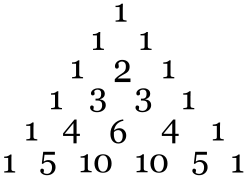
\includegraphics[width=.5\linewidth]{./pascal.png}
\end{center}
\p
فرض کنید
$k_{i,j}$
مقدار 
$j$ام
از سمت چپ در سطر
$i$ام
باشد که شمارنده‌ها از صفر آغاز شوند. برای ساختن این مثلث دو نکته‌ای زیر لازم و کافی است :
\begin{enumerate}
  \item 
  به ازای هر
  $i$
  داریم :
  \begin{center}
    $k_{i,0} = k_{i,i} = 1$
  \end{center}

  \item 
  به ازای هر 
  $i$ و هر
  $0 < j < i$
  داریم :
  \begin{center}
    $k_{i,j} = k_{i-1,j-1} + k_{i-1,j}$
  \end{center}
\end{enumerate}
\p
نکته جالب درمورد این مثلث آن است که اگر قرار دهیم
$$k_{i,j} = {i \choose j}$$
آنگاه می‌دانیم که
$$k{i,0} = {i \choose 0} = 1$$
$$k{i,i} = {i \choose i} = 1$$
و طبق اتحاد پاسکال داریم:
$$k_{i,j} = {i \choose j} = {i-1 \choose j-1} + {i-1 \choose j} = k_{i-1,j-1} + k_{i-1,j}$$

بنابراین می‌توان نتیجه گرفت عضو
$k_{i,j}$
مقدار 
$j$ام
از سمت چپ در سطر
$i$ام
وقتی که شمارنده‌ها از صفر آغاز شوند، برابر 
$i \choose j$
است.